{
\begin{figure*}[th]
\begin{center}
\centerline{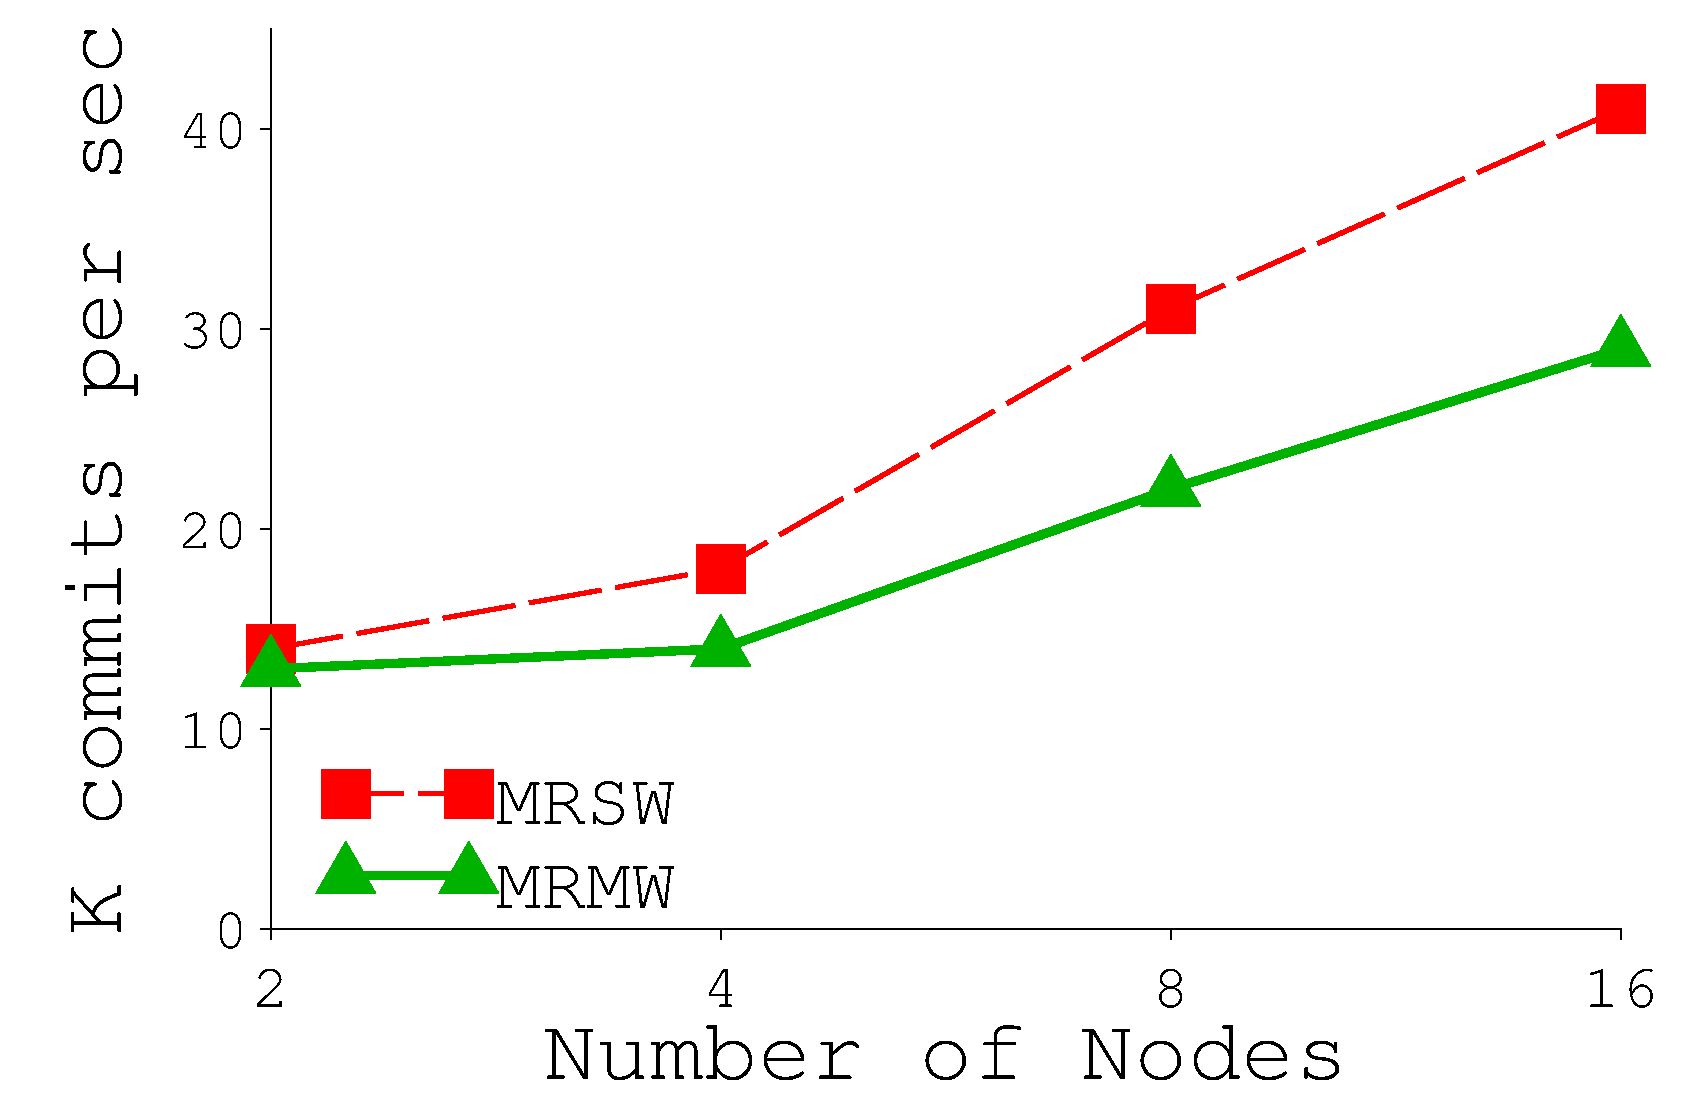
\includegraphics[width=0.6\textwidth]{hotpot/Figures/g_plot_SOCC_node.pdf}}
\caption[\hotpot\ Scalability.]
{
\hotpot\ Scalability.
Commit throughput with 2 to 16 nodes.
}
\label{fig-nodescale}
\end{center}
\end{figure*}
}
{
\begin{figure*}[h]
\begin{center}
\centerline{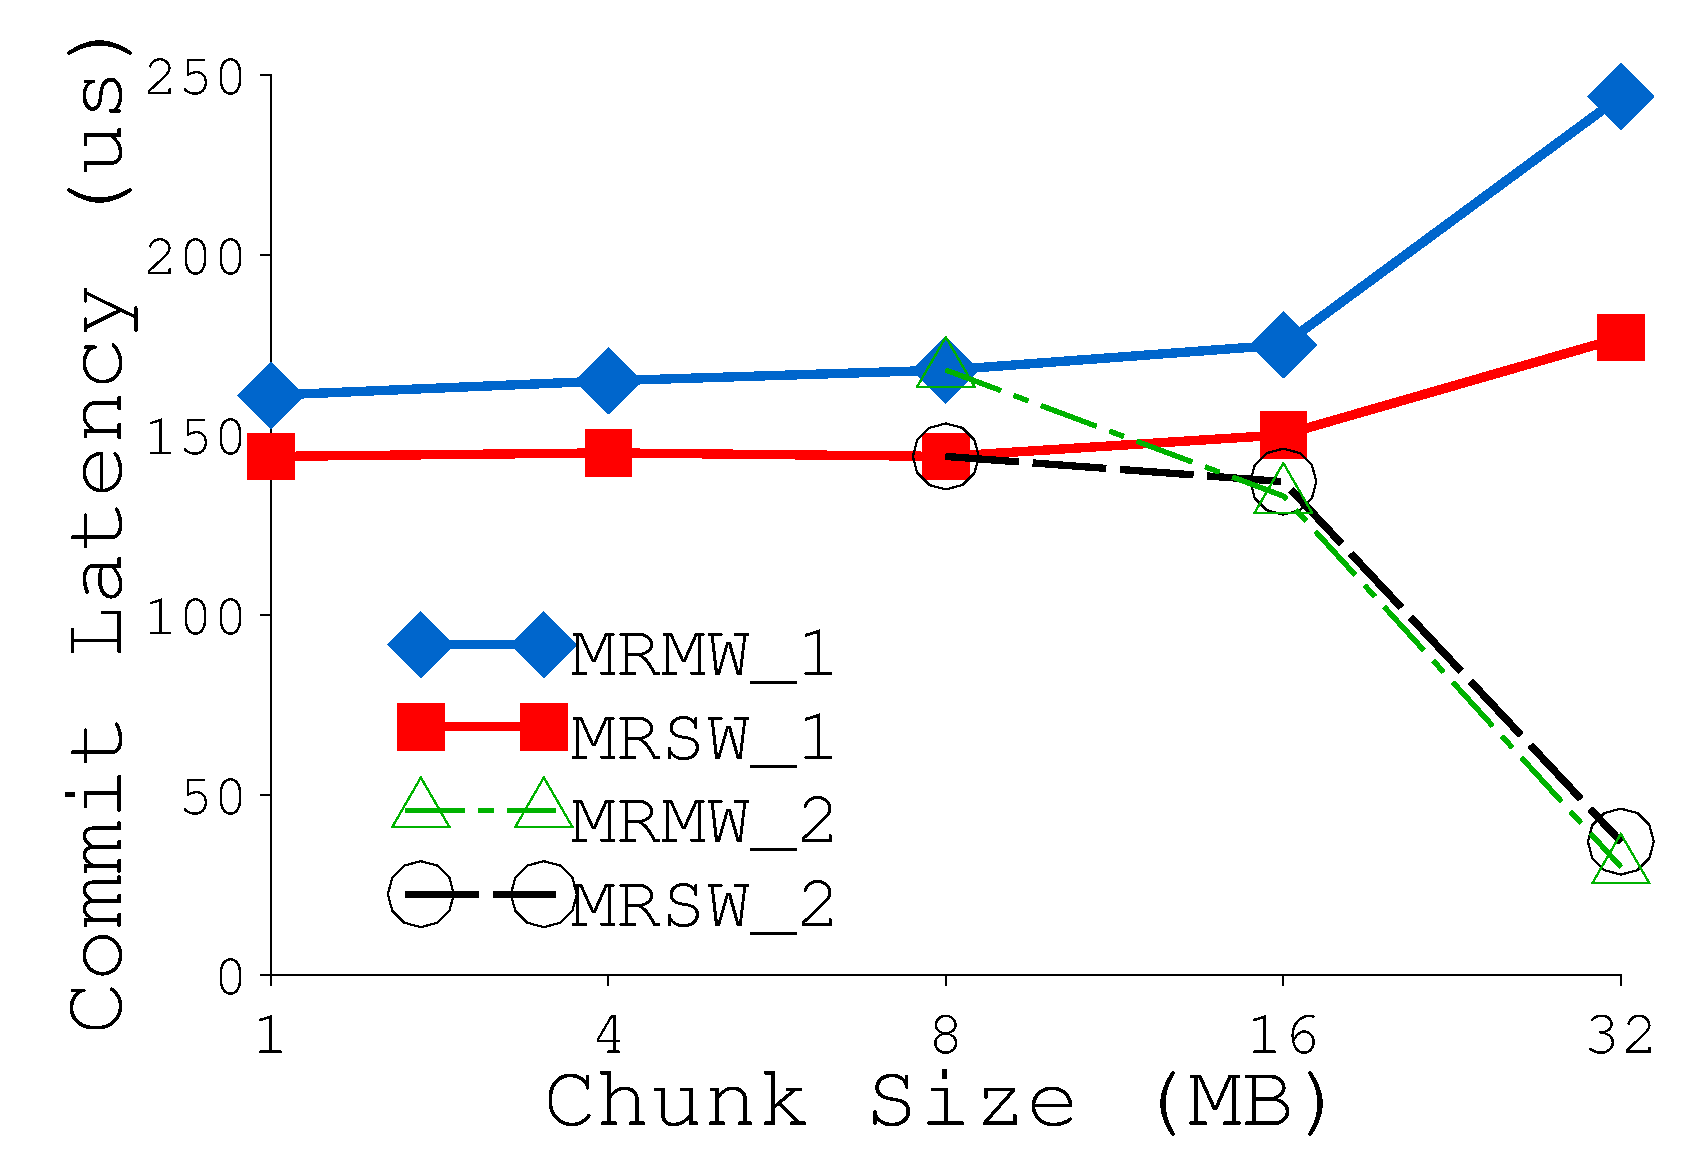
\includegraphics[width=0.6\textwidth]{hotpot/Figures/g_plot_SOCC_chunksize.pdf}}
\caption[Chunk Size.]
{
Chunk Size.
For 16\MB\ and 32\MB\ cases, 1 represents \on\ being remote and 2 represents \xn\ being \on. 
}
\label{fig-chunksize}
\end{center}
\end{figure*}
}
{
\begin{figure*}[h]
\begin{center}
\centerline{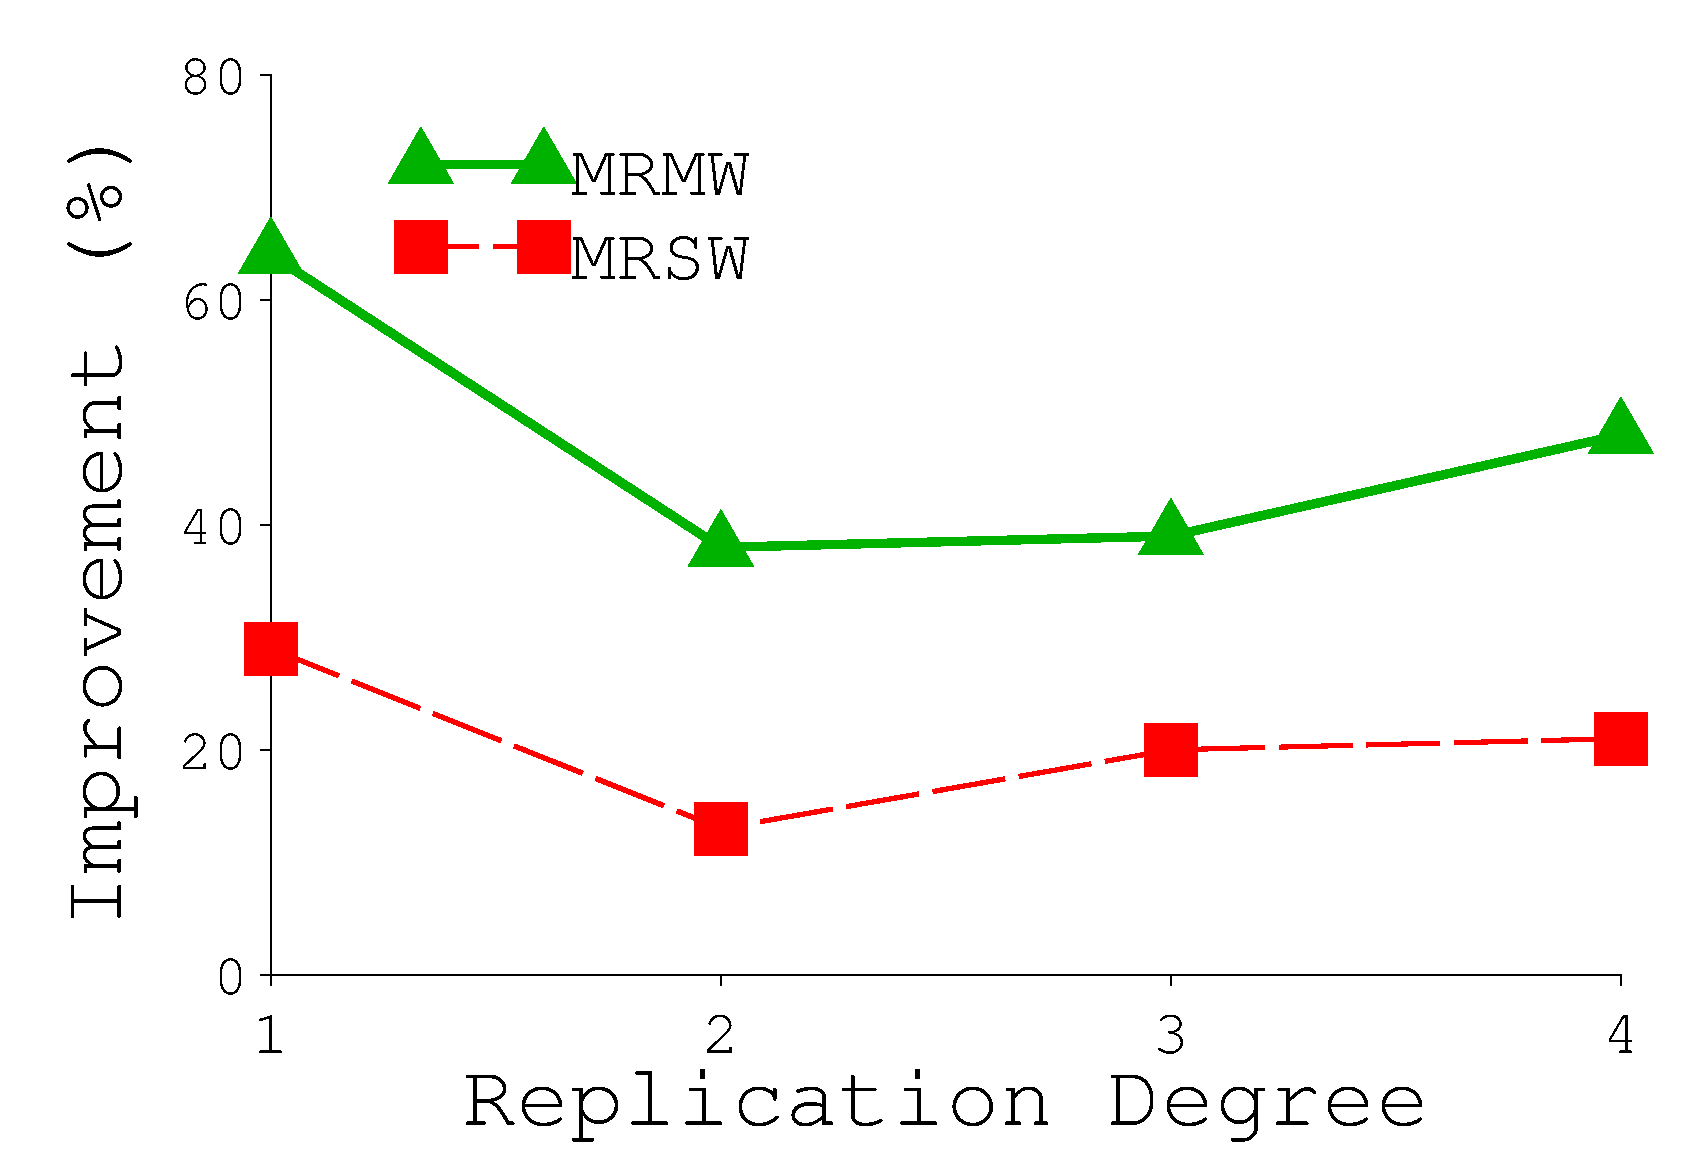
\includegraphics[width=0.6\textwidth]{hotpot/Figures/g_plot_SOCC_migration.pdf}}
\caption[\on\ Migration.]
{
\on\ Migration.
The improvement of average commit latency with \on\ migration over no migration.
}
\label{fig-migration}
\end{center}
\end{figure*}
}
{
\begin{figure*}[h]
\begin{center}
\centerline{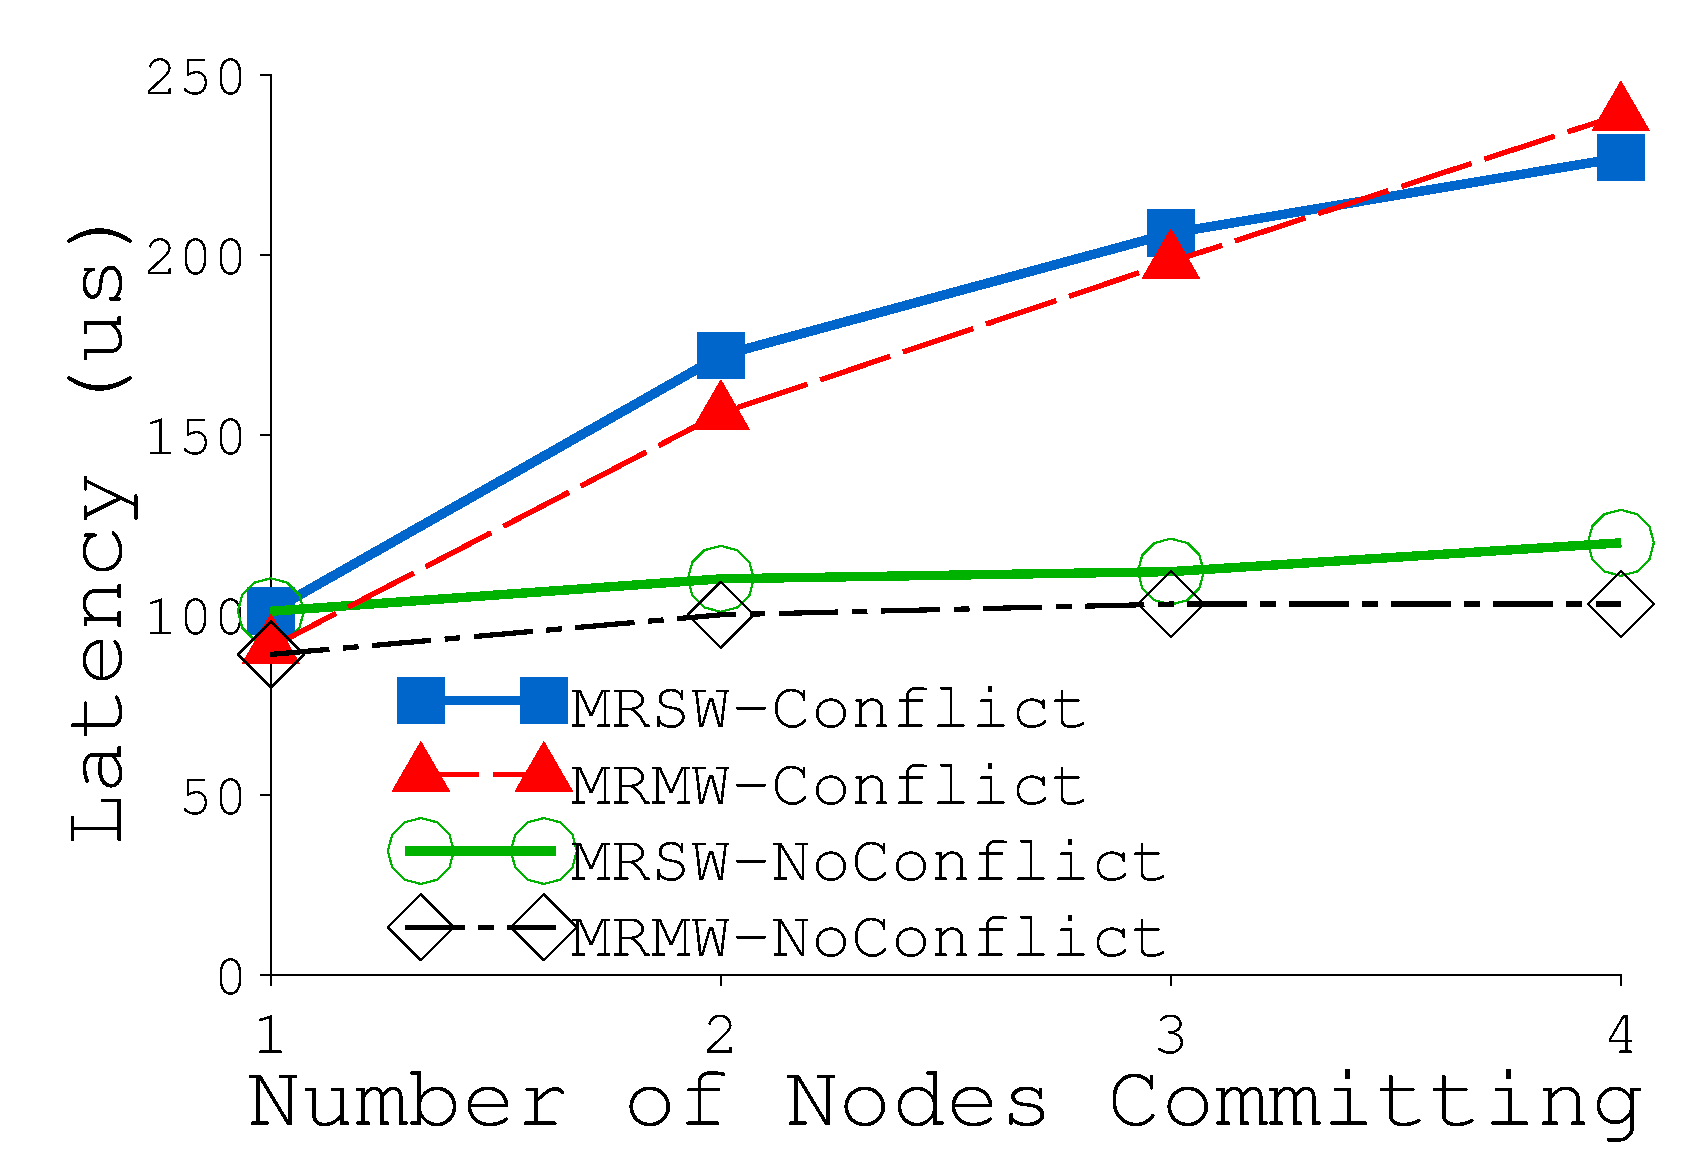
\includegraphics[width=0.6\textwidth]{hotpot/Figures/g_plot_SOCC_conflict.pdf}}
\caption[Commit Conflict.]
{
Commit Conflict.
Average commit latency with and without conflict.
}
\label{fig-conflict}
\end{center}
\end{figure*}
}

\subsection{Micro-Benchmark Results}
\label{sec:hotpot:results}

We now present our microbenchmark results that evaluate the effect of different system settings and parameters.
Since \hotpot\ reads have a constant latency (around 7.9\us) and \hotpot\ writes do not go through network,
\hotpot's performance is largely affected by its data commit process.
Because of space reasons, we focus our microbenchmark experiments on commit.

{\bf Scalability.}
Figure \ref{fig-nodescale} shows the total commit throughput of \hotpot\ on 2 to 16 nodes with a workload 
that lets all nodes concurrently commit 32 random 4\KB\ areas with replication degree 1. 
Overall, both \mrmw\ and \mrsw\ commit scale.
As expected, \mrmw\ \commitxact\ is more costly than \mrsw. 

{\bf Replication degree and committing size.} 
%Figure \ref{fig-repdegree}
We next evaluate the effect of replication degree and the total amount of data in a \commitxact\ call.
%using a workload that let four nodes concurrently commit 32 sequential 4\KB\ areas. 
As expected, with higher replication degree and with more committing data, \commitxact\ takes longer for both \mrmw\ and \mrsw.
%since more replica needs to be made.
Because of space reasons, we do not include figures for these experiments.

{\bf Chunk size.}
We use a controlled microbenchmark to showcase the effect of chunk size (Figure~\ref{fig-chunksize}).
Each run has one node in a cluster of four nodes committing 32 1\KB\ areas that span a 32\MB\ region evenly with replication degree 1.
Since \hotpot\ distributes chunks in Round Robin, 
when chunk size is below 8\MB, the 32\MB\ region will be distributed equally to all four nodes.
The \commitxact\ performance stays similar with 1, 4, and 8\MB\ chunk size,
since \commitxact\ will always use all four nodes as \on{}s.
When chunk size is 16\MB\ (or 32\MB), only two (or one) nodes are \on.
We observe two different behaviors:
when the \xn\ happens to also be the \on\ of the chunk that contains the committing data,
the \commitxact\ performance is better than when chunk size is below 8\MB, since half (or all) commit happens locally at the \xn.
But when the \xn\ is not \on, all commit traffic goes to only two (or one) remote nodes,
resulting in worse performance than when chunk size is small.
This result suggest that smaller chunk size has better load balancing.

{\bf \on\ migration.}
From the previous experiments, we find that the \commitxact\ performance depends heavily on the location of \on\
and the initial \hotpot\ \on\ assignment may not be optimal.
We now evaluate how effective \hotpot's \on\ migration technique is in improving \commitxact\ performance (Figure~\ref{fig-migration}). 
We ran a workload with Zipf distribution to model temporal locality in datacenter applications~\cite{Atikoglu12,Breslau99} on four nodes with replication degree 1 to 4.
Each node issues 100,000 \commitxact\ calls to commit two locations generated by Zipf.
With \on\ migration, the \commitxact\ performance improves by 13\% to 29\% under \mrsw\ and 38\% to 64\% under \mrmw.
\on\ migration improves performance because the node that performs most \commitxact\ on a chunk becomes its \on\ after migration.
The improvement is most significant with replication degree one, 
because when \xn\ is \on\ and replication degree is one, there is no need to perform any network communication.
\mrmw's improvement is higher than \mrsw, because \mrmw\ can benefit more from committing data locally
--- the \mrmw\ commit process that involves remote \on{}s is more costly than that of \mrsw.

{\bf Effect of conflict commits.}
Figure~\ref{fig-conflict} compares the \commitxact\ performance of when 1 to 4 nodes in a four node cluster 
concurrently commit data in two scenarios:
all \xn{}s commit the same set of data (32 sequential 1\KB\ areas) at the same time which results in commit conflict,
%and synchronizes all nodes the commit at the same time, resulting in commit conflict.
and \xn{}s use different set of data without any conflict.
Commit conflict causes degraded performance, 
and the degradation is worse with more conflicting nodes.
However, conflict is rare in reality, since \commitxact\ is fast.
Conflict only happens when different nodes commit the same data page at exactly the same time.
In fact, we had to manually synchronize all nodes at every \commitxact\ call using \barrier\ to create conflict.
